\documentclass{standalone}
\usepackage{tikz}
\usetikzlibrary{shapes, calc}



\begin{document}


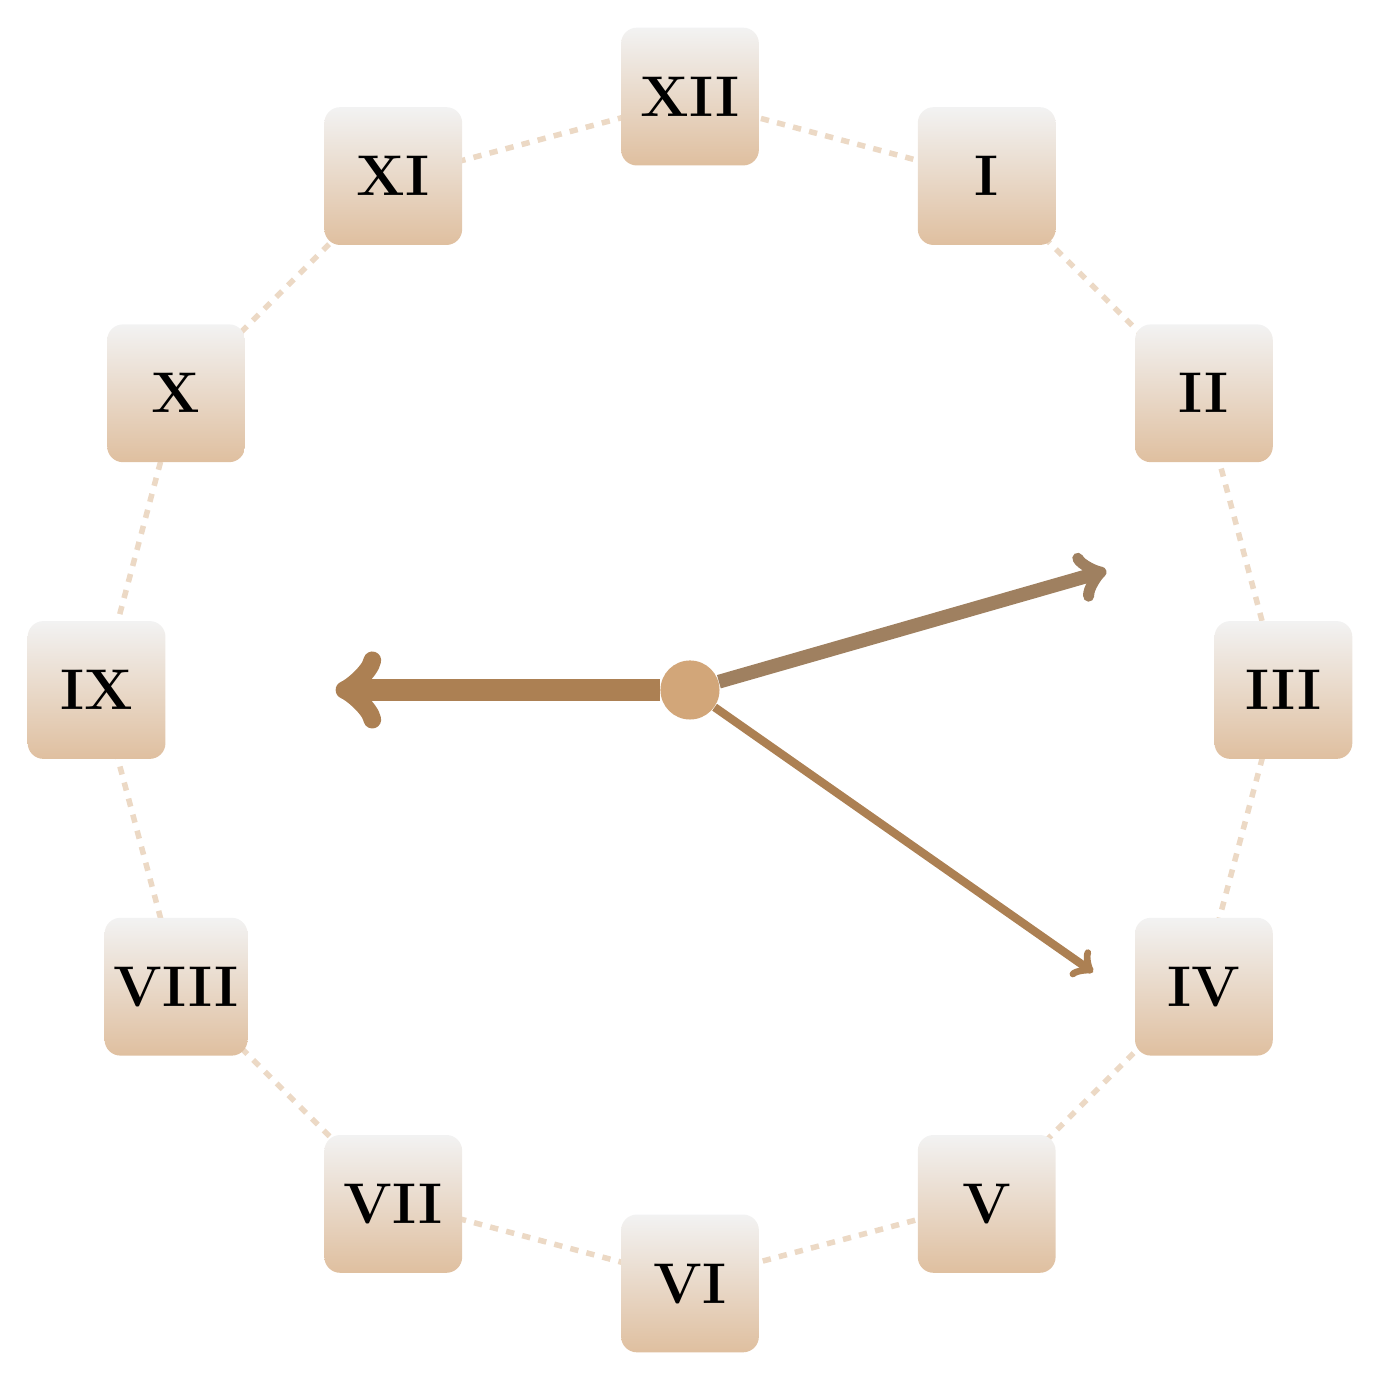
\begin{tikzpicture}[
vertex_style/.style={circle,shading=ball,ball color=red,draw=red!80!white,drop shadow={opacity=0.4}},
node_spin/.style={circle, shading=ball, ball color=gray!10!white, draw=none, minimum width=1.5cm,inner sep=0.1cm, opacity=0.7},
edge_style/.style={ultra thick, black,drop shadow={opacity=0.4}},
		hora/.style={rectangle, minimum width=1.75cm, minimum height=1.75cm, rounded corners=2mm, top color=gray!10, bottom color=brown!50}, font=\huge \bfseries, 
		]
 
\begin{scope}[xshift=0cm, rotate=0]

	\def\lados{12};
	\node[regular polygon, regular polygon sides=\lados, minimum size=15.cm, draw=brown, dashed, line width=2pt, rotate=15, transform shape, opacity=0.3] at (0,0) (polygonnode) {};
	
	\node[hora] at (polygonnode.corner 1) (xii) []{XII};
	\node[hora] at (polygonnode.corner 2) (xi) []{XI};
	\node[hora] at (polygonnode.corner 3) (x) []{X};
	\node[hora] at (polygonnode.corner 4) (ix) []{IX};
	\node[hora] at (polygonnode.corner 5) (viii) []{VIII};   
	\node[hora] at (polygonnode.corner 6) (vii) []{VII};
	\node[hora] at (polygonnode.corner 7) (vi) []{VI};	
	\node[hora] at (polygonnode.corner 8) (v) []{V};
	\node[hora] at (polygonnode.corner 9) (iv) []{IV};
	\node[hora] at (polygonnode.corner 10) (iii) []{III};
	\node[hora] at (polygonnode.corner 11) (ii) []{II};
	\node[hora, anchor=center] at (polygonnode.corner 12) (i) []{I};
	
	\node[circle, fill=brown, minimum width=0.75cm, opacity=0.7] (centroponteiro) at (polygonnode.center) {};
	
	
	
	\draw[->, color=brown!50!gray, line width=5pt, rotate=-74] (centroponteiro)--($(centroponteiro)+(0, 5.5)$) node(ponteiromin){} ;
	
	\draw[->, color=brown!70!gray, line width=8pt, rotate=90] (centroponteiro)--($(centroponteiro)+(0, 4.5)$) node(ponteirohora) {} ;
	
	\draw[->, color=brown!70!gray, line width=3pt, rotate=235] (centroponteiro)--($(centroponteiro)+(0, 6.25)$) node(ponteirosegundos) {} ;
	
	%\node[inner sep=0mm] (desenho) at ($(centroponteiro)+(0.25, 0.5)$) {\includegraphics[scale=0.15]{figs/surprise1.png}};
	
	%\node[inner sep=0mm] (desenho2) at ($(centroponteiro)+(3.5,3.5)$) {\includegraphics[scale=0.25]{figs/surprise2.png}};
	
	%\node[inner sep=0mm] (desenho3) at ($(centroponteiro)+(-2.5,-3.5)$) {\includegraphics[scale=0.35]{figs/surprise3.png}};
	%\node[inner sep=0mm, font=\huge \bfseries] (desenho3t) at ($(desenho3.north)+(0,0.5)$) {coffee time???};

	
\end{scope}

\end{tikzpicture}


\end{document}
